\subsection{Frequency Noise}
In this section image 4.1 is considered.
As the image contains a lot of lines, a frequency analysis of the image was made.
The magnitude plot of this is seen in figure \ref{fig:freq_analysis_p4}.


\begin{figure}[H]
\centering
\begin{tikzpicture}

\node {\centering \includegraphics[width = 0.9 \linewidth]{../code/images/frequency_analysis_04.png}};

\node[circle, draw, minimum width = 0.4cm,red,very thick] at (1.45, 1.41) {};

\node[circle, draw, minimum width = 0.3cm,red,very thick] at (0.54, -0.48) {};

\end{tikzpicture}

\caption{Magnitude plot of image 4.1 in the frequency domain.}
\label{fig:freq_analysis_p4}
\end{figure}




In figure \ref{fig:freq_analysis_p4}, two pairs of bright spots can be seen were one from the pair is marked by a red circle.
These two pairs originate from the 




\begin{figure}[H]
\centering
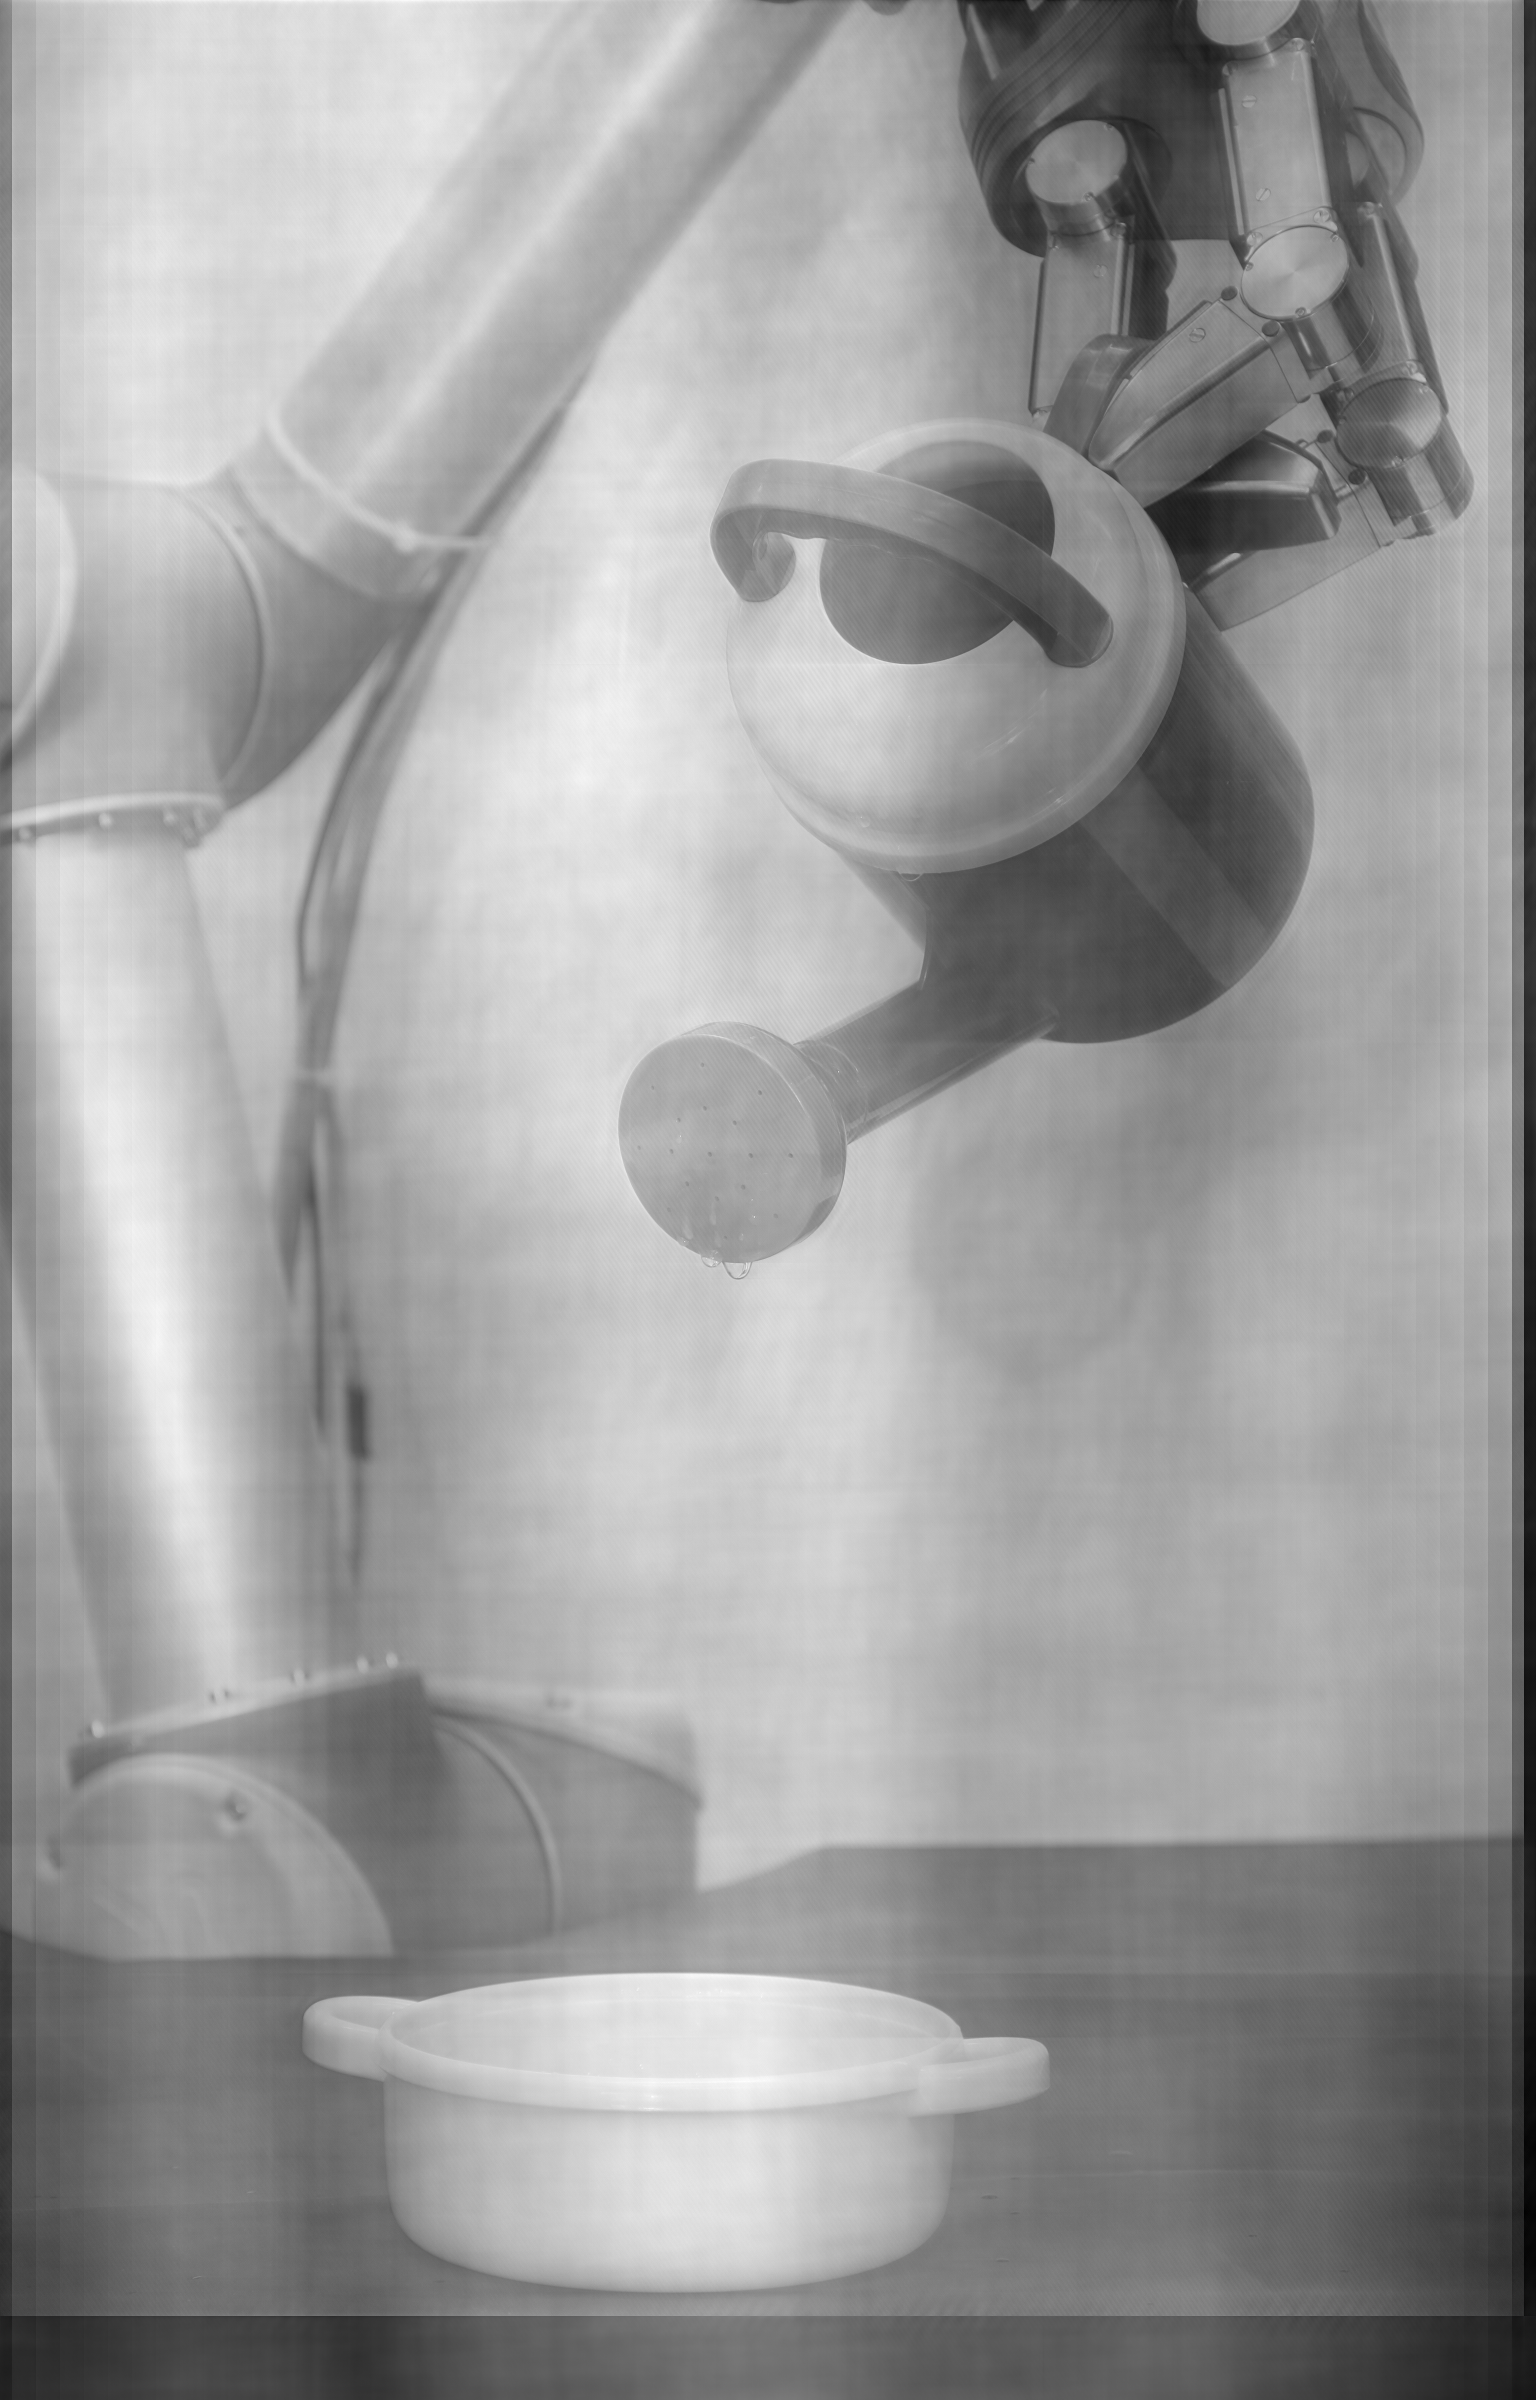
\includegraphics[width = 0.9 \linewidth]{../code/images/image_result_04.png}
\caption{Resulting image after filtering in the frequency domain.}
\label{fig:hist_pepper}
\end{figure}
